% !TEX root = smc_bandits.tex

\subsection{Experiments with SMC-based Bayesian policies for logistic stationary bandits}
\label{assec:static_bandits_experiments_logistic}

Results in Sections~\ref{asssec:static_bandits_logistic_2} and \ref{asssec:static_bandits_logistic_5}
demonstrate how SMC-based Thompson sampling and Bayes-UCB achieve
successful exploration-exploitation tradeoff, 
for different parameterizations of stationary logistic bandits.
%
This evidence indicates that
the impact of observing context-dependent binary rewards of the played arms is minimal for the proposed SMC-based policies.

The parameter posterior uncertainty associated with SMC-based estimation
is automatically accounted for by both algorithms,
as they explore rarely-played arms if the uncertainty is high.
However, we observe a slight performance deterioration for SMC-based Bayes-UCB,
which we hypothesize is related to the quantile value used ($\alpha_t\propto1/t$).
This decay rate was justified by Kaufmann~\cite{ip-Kaufmann2012} for Bernoulli rewards,
but might not be optimal for other reward functions and,
more importantly, for the SMC-based parameter posterior random measures.

On the contrary, Thompson sampling automatically adjusts
to the uncertainty of the posterior random measure without extra hyperparameter search or tuning,
and attains reduced regret.

\subsubsection{Contextual logistic bandits, A=2}
\label{asssec:static_bandits_logistic_2}

We present below cumulative regret results for different parameterizations of 2-armed, contextual logistic bandits.

% theta-0.1_-0.1_0.1_0.1
\begin{figure}[!h]
	\centering
	\begin{subfigure}[b]{\textwidth}
		\centering
		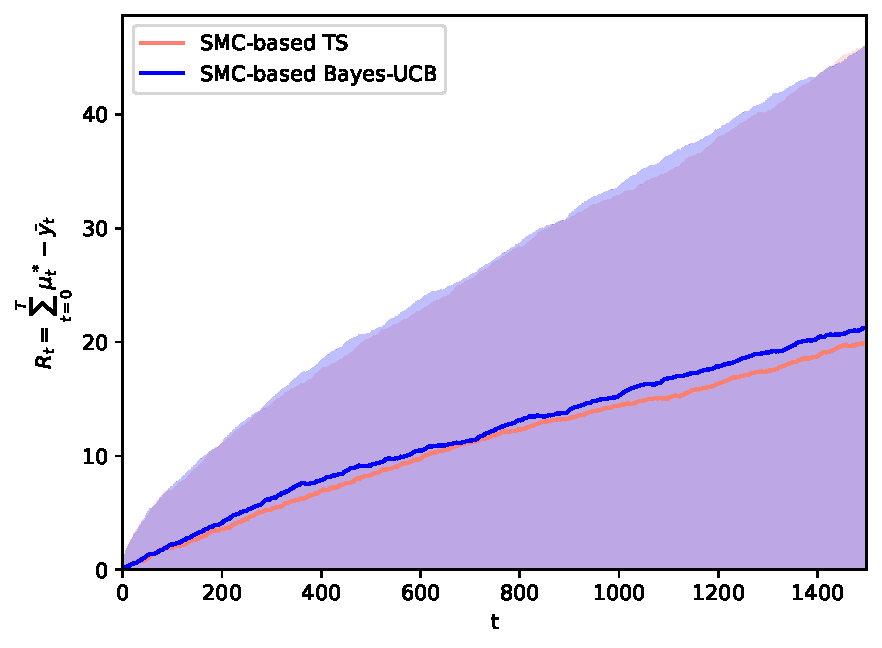
\includegraphics[width=0.75\textwidth]{./fods_figs/static/logistic/A2/theta-0.1_-0.1_0.1_0.1_M1000_cumulative_regret}
		\caption{SMC-based ($M=1000$) TS and Bayes-UCB.}
	\end{subfigure}
	
	\begin{subfigure}[b]{0.46\textwidth}
		\centering
		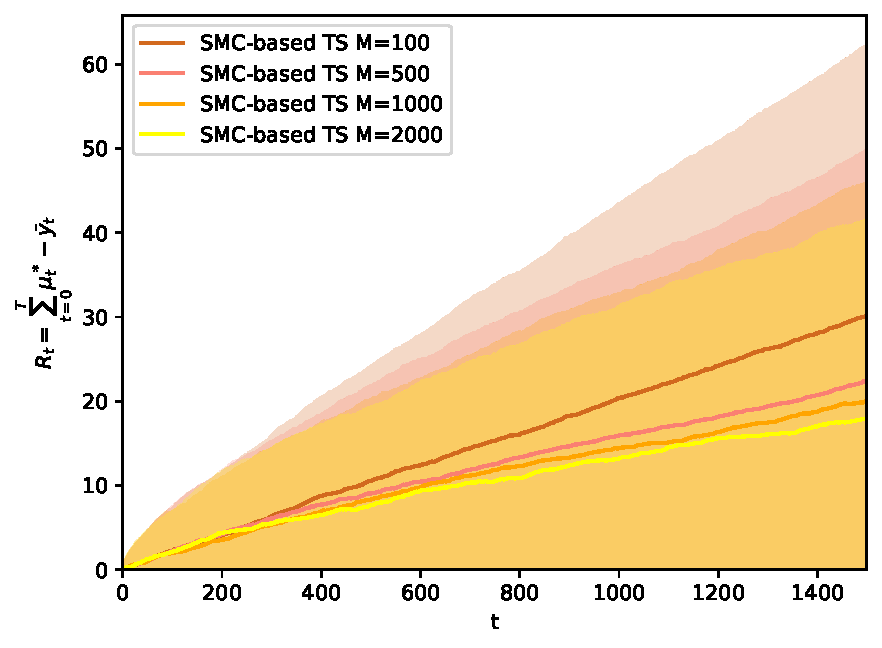
\includegraphics[width=\textwidth]{./fods_figs/static/logistic/A2/theta-0.1_-0.1_0.1_0.1_allM_cumulative_regret_ts}
		\caption{SMC-based TS: impact of $M$.}
	\end{subfigure}
	\begin{subfigure}[b]{0.46\textwidth}
		\centering
		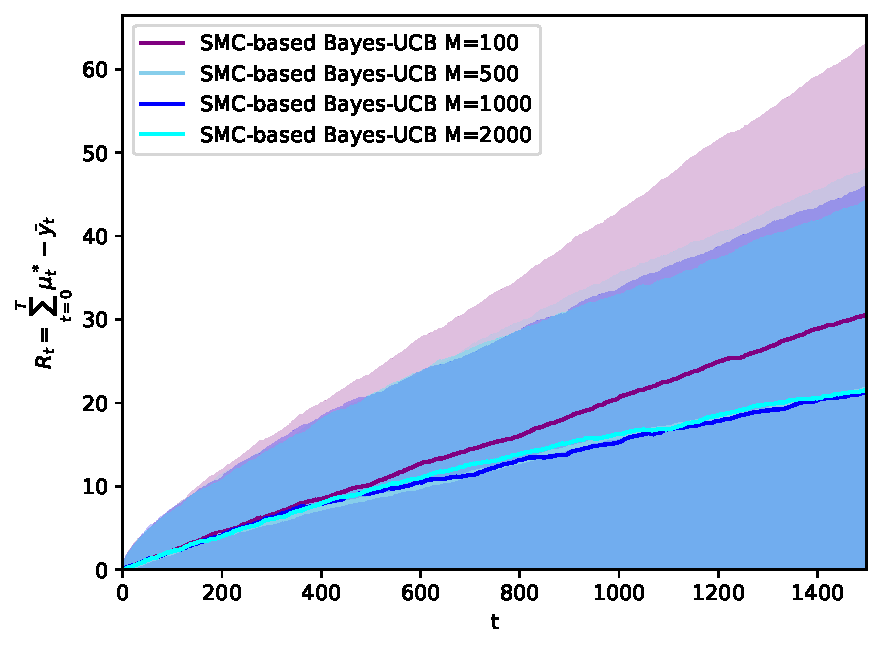
\includegraphics[width=\textwidth]{./fods_figs/static/logistic/A2/theta-0.1_-0.1_0.1_0.1_allM_cumulative_regret_bucb}
		\caption{SMC-based Bayes-UCB: impact of $M$}
	\end{subfigure}
	
	\caption{Mean cumulative regret (standard deviation shown as the shaded region) of SMC-based Bayesian policies in
		stationary, two-armed contextual logistic bandits:
		$\theta_0=(-0.1,-0.1), \ \theta_1=(0.1,0.1)$.}
\end{figure}

% theta-0.5_-0.5_0.5_0.5
\begin{figure}[!h]
	\centering
	\begin{subfigure}[b]{\textwidth}
		\centering
		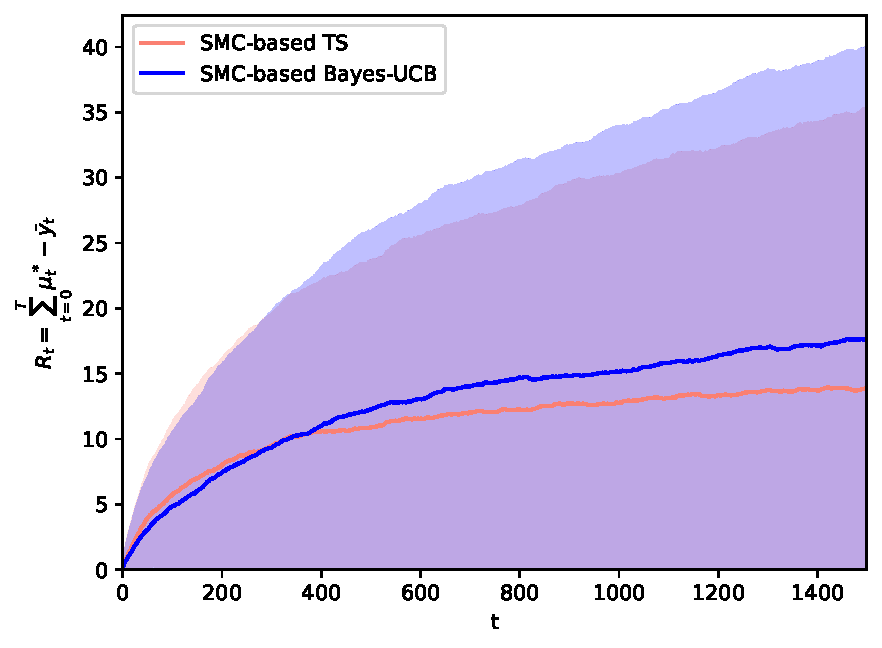
\includegraphics[width=0.75\textwidth]{./fods_figs/static/logistic/A2/theta-0.5_-0.5_0.5_0.5_M1000_cumulative_regret}
		\caption{SMC-based ($M=1000$) TS and Bayes-UCB.}
	\end{subfigure}
	
	\begin{subfigure}[b]{0.46\textwidth}
		\centering
		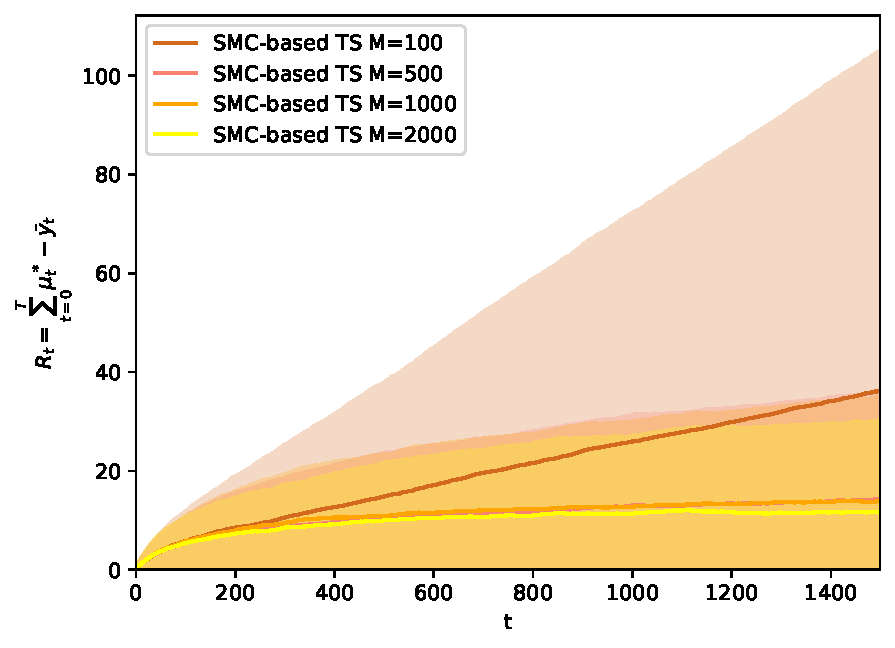
\includegraphics[width=\textwidth]{./fods_figs/static/logistic/A2/theta-0.5_-0.5_0.5_0.5_allM_cumulative_regret_ts}
		\caption{SMC-based TS: impact of $M$.}
	\end{subfigure}
	\begin{subfigure}[b]{0.46\textwidth}
		\centering
		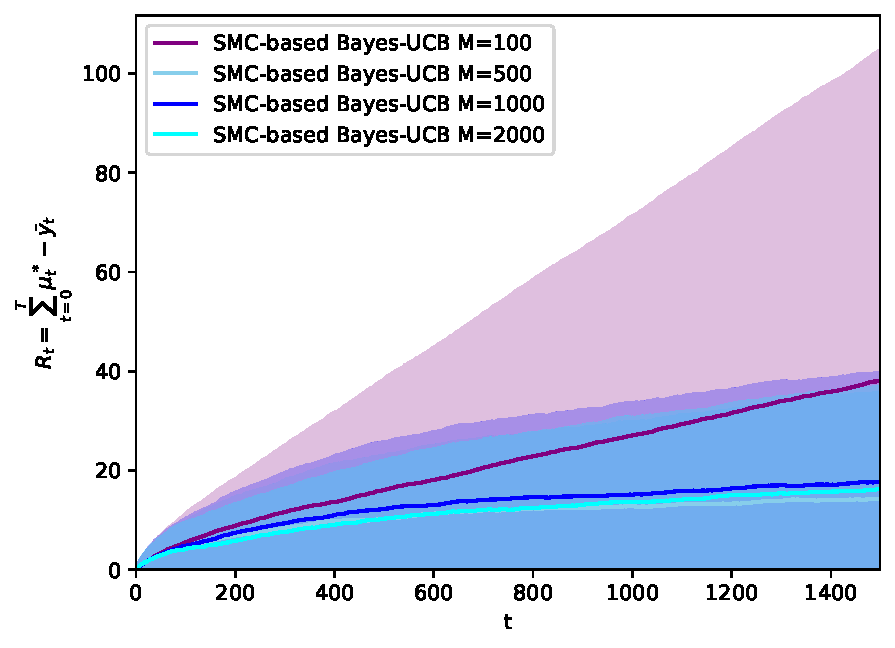
\includegraphics[width=\textwidth]{./fods_figs/static/logistic/A2/theta-0.5_-0.5_0.5_0.5_allM_cumulative_regret_bucb}
		\caption{SMC-based Bayes-UCB: impact of $M$}
	\end{subfigure}
	
	\caption{Mean cumulative regret (standard deviation shown as the shaded region) of SMC-based Bayesian policies in
		stationary, two-armed contextual logistic bandits:
		$\theta_0=(-0.5,-0.5), \ \theta_1=(0.5,0.5)$.}
\end{figure}

% theta-1._-1._1._1.
\begin{figure}[!h]
	\centering
	\begin{subfigure}[b]{\textwidth}
		\centering
		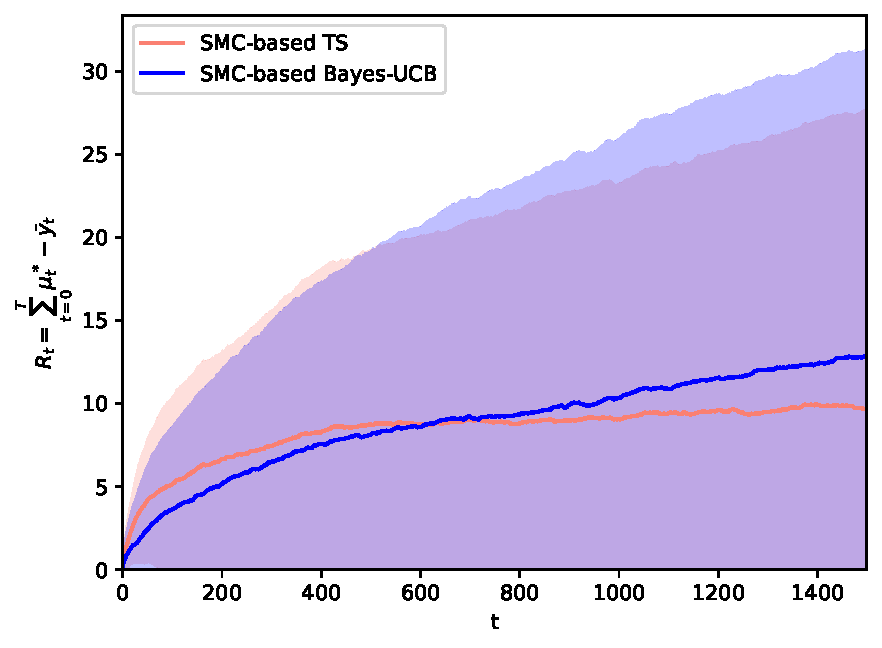
\includegraphics[width=0.75\textwidth]{./fods_figs/static/logistic/A2/theta-1._-1._1._1._M1000_cumulative_regret}
		\caption{SMC-based ($M=1000$) TS and Bayes-UCB.}
	\end{subfigure}
	
	\begin{subfigure}[b]{0.46\textwidth}
		\centering
		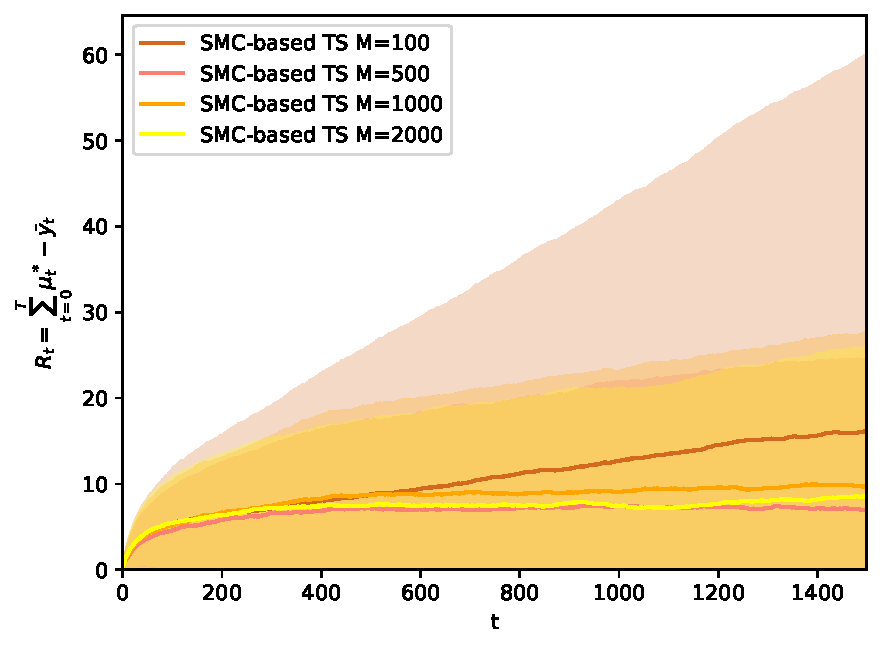
\includegraphics[width=\textwidth]{./fods_figs/static/logistic/A2/theta-1._-1._1._1._allM_cumulative_regret_ts}
		\caption{SMC-based TS: impact of $M$.}
	\end{subfigure}
	\begin{subfigure}[b]{0.46\textwidth}
		\centering
		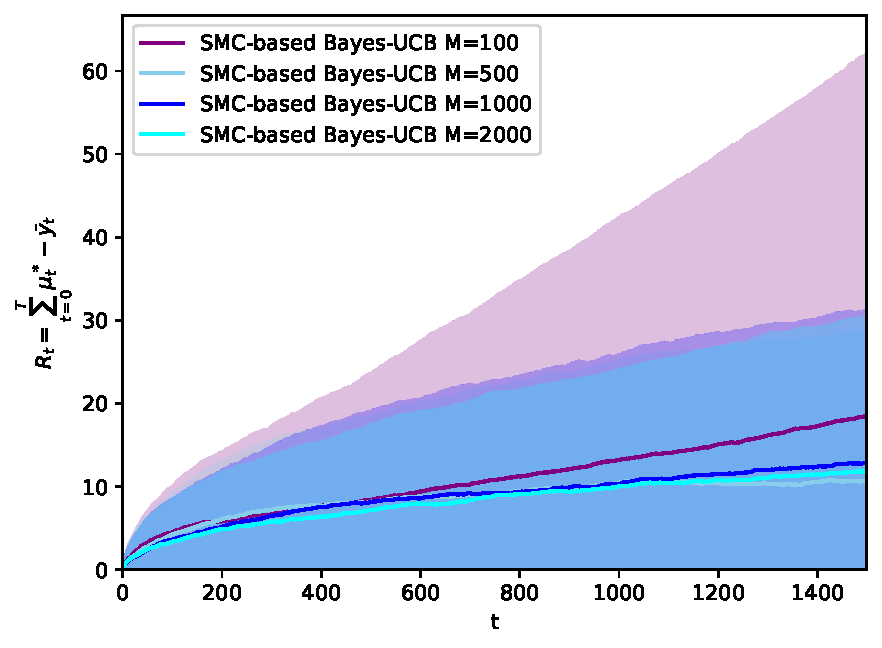
\includegraphics[width=\textwidth]{./fods_figs/static/logistic/A2/theta-1._-1._1._1._allM_cumulative_regret_bucb}
		\caption{SMC-based Bayes-UCB: impact of $M$}
	\end{subfigure}
	
	\caption{Mean cumulative regret (standard deviation shown as the shaded region) of SMC-based Bayesian policies in
		stationary, two-armed contextual logistic bandits:
		$\theta_0=(-1.0,-1.0), \ \theta_1=(1.0,1.0)$.}
\end{figure}

\clearpage
\subsubsection{Contextual logistic bandits, A=5}
\label{asssec:static_bandits_logistic_5}

We present below cumulative regret results for different parameterizations of 5-armed, contextual logistic bandits.

% theta-0.2_-0.2_-0.1_-0.1_0._0._0.1_0.1_0.2_0.2
\begin{figure}[!h]
	\centering
	\begin{subfigure}[b]{\textwidth}
		\centering
		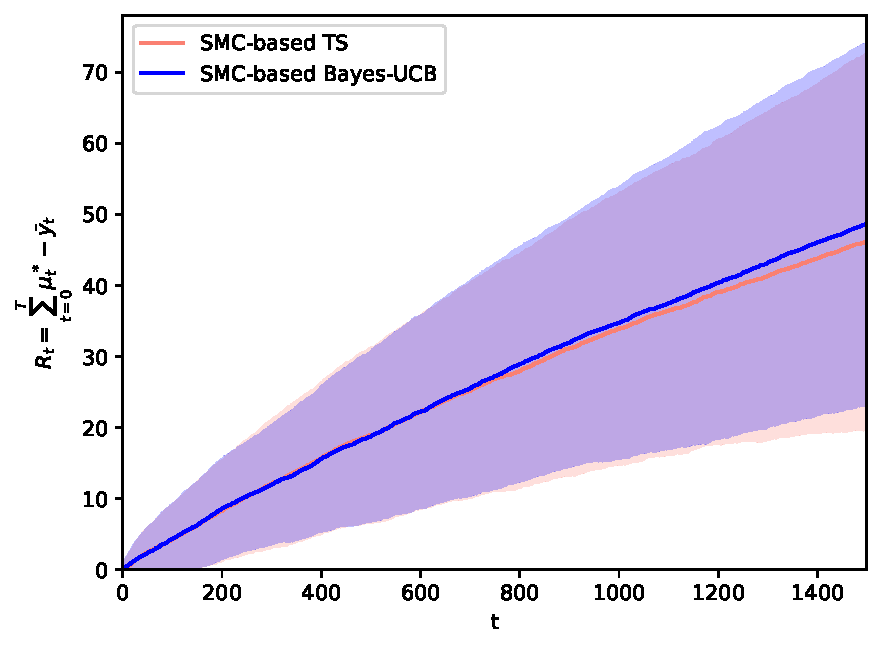
\includegraphics[width=0.75\textwidth]{./fods_figs/static/logistic/A5/theta-0.2_-0.2_-0.1_-0.1_0._0._0.1_0.1_0.2_0.2_M1000_cumulative_regret}
		\caption{SMC-based ($M=1000$) TS and Bayes-UCB.}
	\end{subfigure}
	
	\begin{subfigure}[b]{0.46\textwidth}
		\centering
		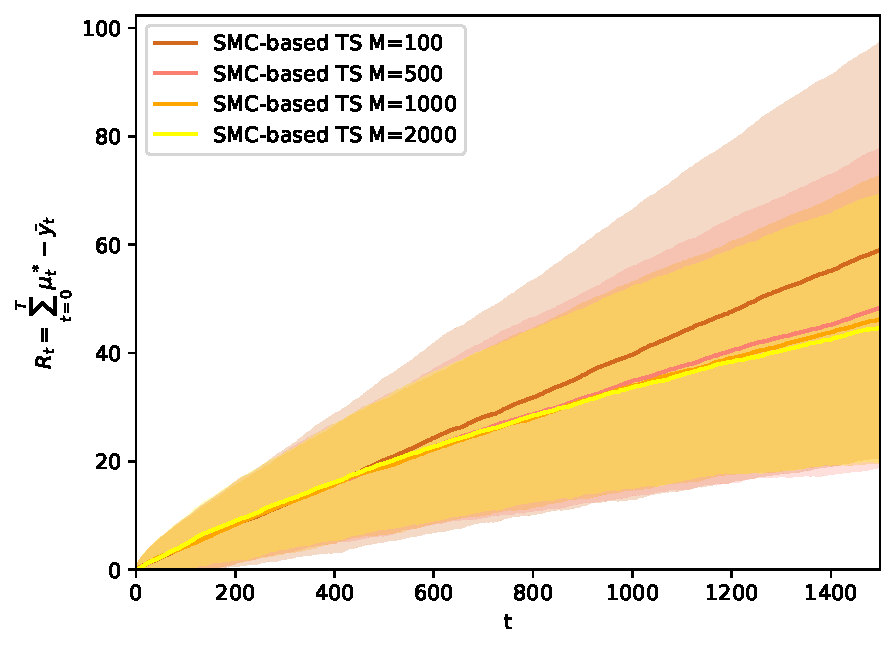
\includegraphics[width=\textwidth]{./fods_figs/static/logistic/A5/theta-0.2_-0.2_-0.1_-0.1_0._0._0.1_0.1_0.2_0.2_allM_cumulative_regret_ts}
		\caption{SMC-based TS: impact of $M$.}
	\end{subfigure}
	\begin{subfigure}[b]{0.46\textwidth}
		\centering
		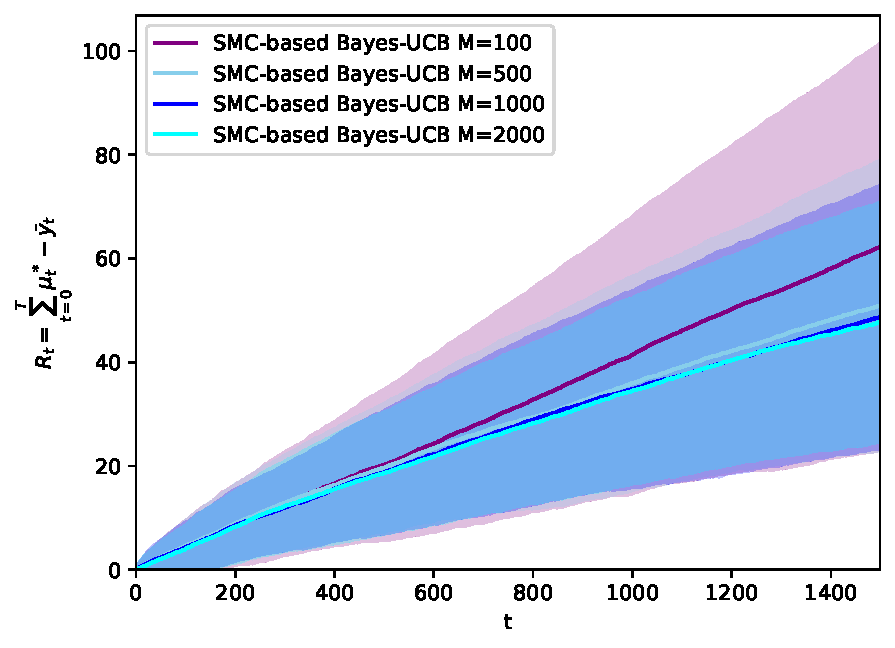
\includegraphics[width=\textwidth]{./fods_figs/static/logistic/A5/theta-0.2_-0.2_-0.1_-0.1_0._0._0.1_0.1_0.2_0.2_allM_cumulative_regret_bucb}
		\caption{SMC-based Bayes-UCB: impact of $M$}
	\end{subfigure}
	
	\caption{Mean cumulative regret (standard deviation shown as the shaded region) of SMC-based Bayesian policies in
		stationary, five-armed contextual logistic bandits:
		$\theta_0=(-0.2,-0.2), \ \theta_1=(-0.1,-0.1), \ \theta_2=(0,0), \ \theta_3=(0.1,0.1), \ \theta_4=(0.2,0.2)$.
	}
\end{figure}

% theta-1._-1._-0.5_-0.5_0._0._0.5_0.5_1._1
\begin{figure}[!h]
	\centering
	\begin{subfigure}[b]{\textwidth}
		\centering
		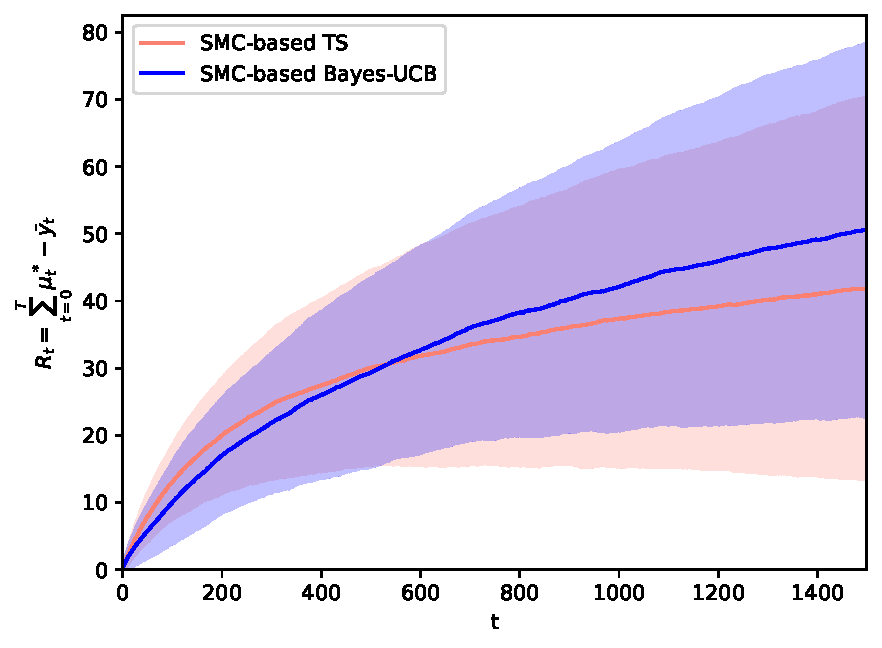
\includegraphics[width=0.75\textwidth]{./fods_figs/static/logistic/A5/theta-1._-1._-0.5_-0.5_0._0._0.5_0.5_1._1._M1000_cumulative_regret}
		\caption{SMC-based ($M=1000$) TS and Bayes-UCB.}
	\end{subfigure}
	
	\begin{subfigure}[b]{0.46\textwidth}
		\centering
		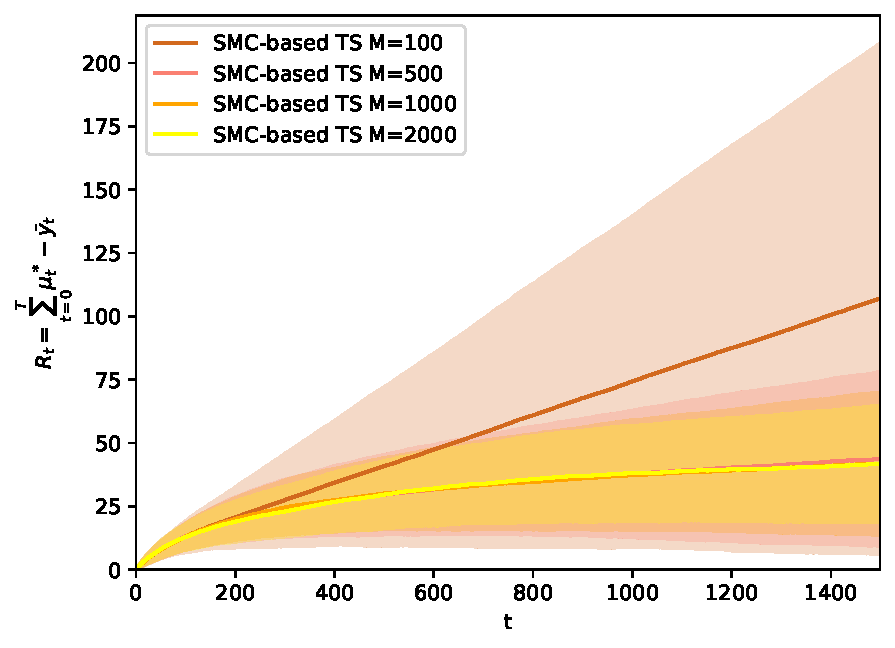
\includegraphics[width=\textwidth]{./fods_figs/static/logistic/A5/theta-1._-1._-0.5_-0.5_0._0._0.5_0.5_1._1._allM_cumulative_regret_ts}
		\caption{SMC-based TS: impact of $M$.}
	\end{subfigure}
	\begin{subfigure}[b]{0.46\textwidth}
		\centering
		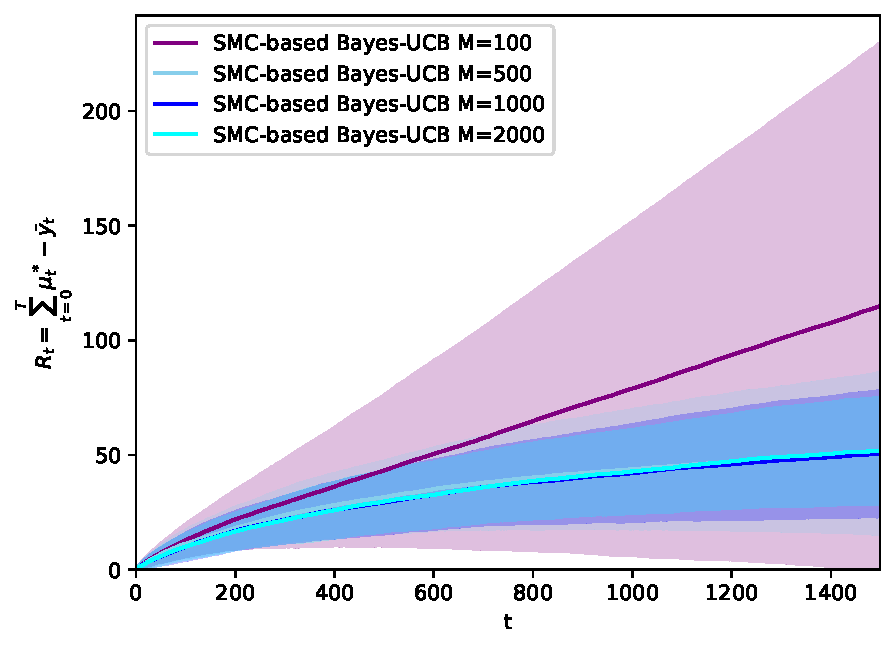
\includegraphics[width=\textwidth]{./fods_figs/static/logistic/A5/theta-1._-1._-0.5_-0.5_0._0._0.5_0.5_1._1._allM_cumulative_regret_bucb}
		\caption{SMC-based Bayes-UCB: impact of $M$}
	\end{subfigure}
	
	\caption{Mean cumulative regret (standard deviation shown as the shaded region) of SMC-based Bayesian policies in
		stationary, five-armed contextual logistic bandits:
		$\theta_0=(-1.0,-1.0), \ \theta_1=(-0.5,-0.5), \ \theta_2=(0,0), \ \theta_3=(0.5,0.5), \ \theta_4=(1.0,1.0)$.
	}
\end{figure}

% theta-2._-2._-1._-1._0._0._1._1._2._2.
\begin{figure}[!h]
	\centering
	\begin{subfigure}[b]{\textwidth}
		\centering
		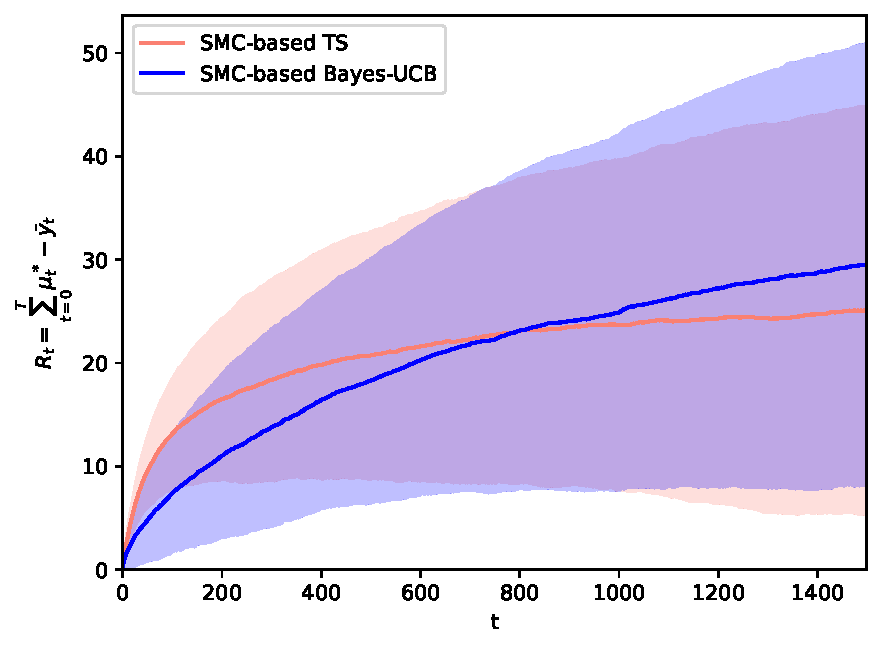
\includegraphics[width=0.75\textwidth]{./fods_figs/static/logistic/A5/theta-2._-2._-1._-1._0._0._1._1._2._2._M1000_cumulative_regret}
		\caption{SMC-based ($M=1000$) TS and Bayes-UCB.}
	\end{subfigure}
	
	\begin{subfigure}[b]{0.46\textwidth}
		\centering
		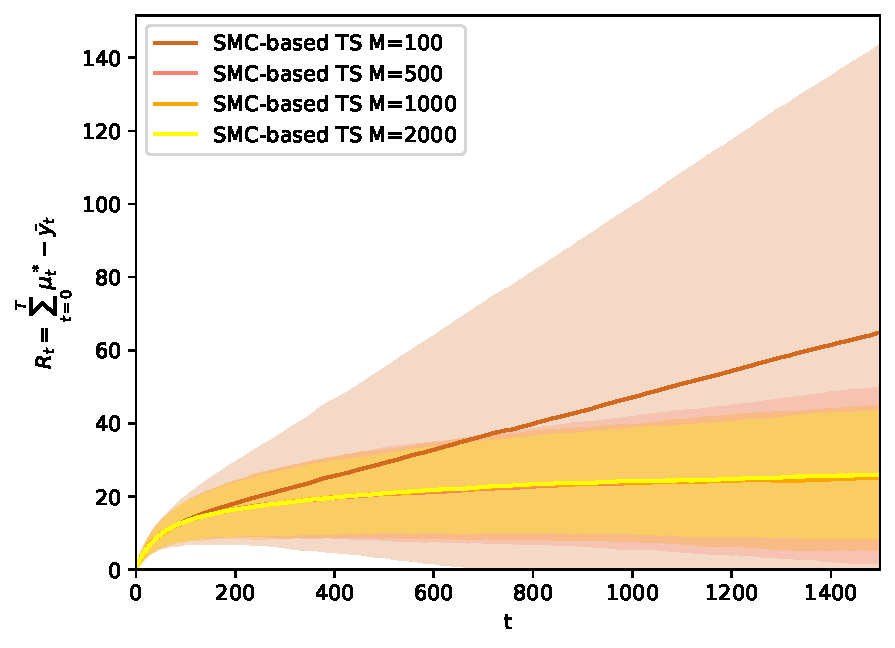
\includegraphics[width=\textwidth]{./fods_figs/static/logistic/A5/theta-2._-2._-1._-1._0._0._1._1._2._2._allM_cumulative_regret_ts}
		\caption{SMC-based TS: impact of $M$.}
	\end{subfigure}
	\begin{subfigure}[b]{0.46\textwidth}
		\centering
		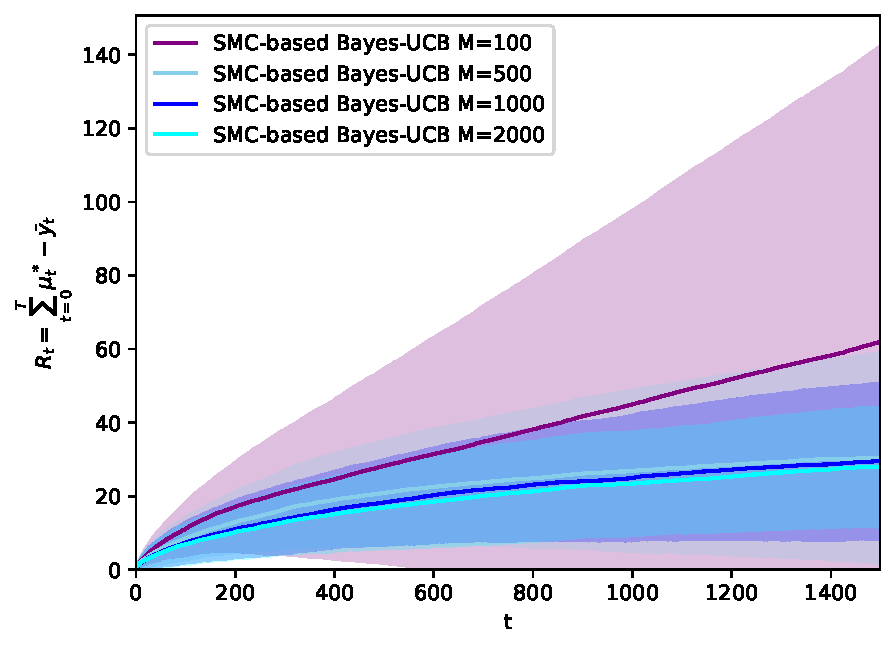
\includegraphics[width=\textwidth]{./fods_figs/static/logistic/A5/theta-2._-2._-1._-1._0._0._1._1._2._2._allM_cumulative_regret_bucb}
		\caption{SMC-based Bayes-UCB: impact of $M$}
	\end{subfigure}
	
	\caption{Mean cumulative regret (standard deviation shown as the shaded region) of SMC-based Bayesian policies in
		stationary, five-armed contextual logistic bandits:
		$\theta_0=(-2.0,-2.0), \ \theta_1=(-1.0,-1.0), \ \theta_2=(0,0), \ \theta_3=(1.0,1.0), \ \theta_4=(2.0,2.0)$.
	}
\end{figure}